\documentclass{article}
\usepackage[utf8]{inputenc}
\usepackage{tikz}
\usepackage{pgfplots}
\pgfplotsset{compat=1.18}
\usetikzlibrary{shapes,arrows,positioning,decorations.pathreplacing}

\title{TikZ Diagrams in LaTeX}
\author{LaTeX Research Toolkit}
\date{\today}

\begin{document}

\maketitle

\section*{Introduction}
This document demonstrates advanced TikZ features for creating complex and visually appealing mathematical graphics and diagrams in \LaTeX. The examples in this document are inspired by Dr. Trefor Bazett's comprehensive TikZ tutorial, which covers everything from basic shapes to advanced node-based diagrams with styled elements and B\'ezier curves.

Key concepts covered include:
\begin{itemize}
    \item Basic shapes and coordinate systems
    \item Styling with colors, fills, and shading
    \item Line styles and arrow variations
    \item Advanced node usage with text and math mode
    \item Relative positioning and anchored nodes
    \item Complex flow diagrams with B\'ezier curves
    \item Reusable custom styles for consistent formatting
\end{itemize}

\section{Basic TikZ Examples}
Here are some basic TikZ diagrams:

\subsection{Simple Shapes}
\begin{tikzpicture}
% Draw a circle
\draw (0,0) circle (1cm);

% Draw a rectangle
\draw (3,0) rectangle (5,2);

% Draw a line
\draw (6,0) -- (8,2);

% Draw an arrow
\draw[->] (9,0) -- (11,2);
\end{tikzpicture}

\subsection{Coordinate System}
\begin{tikzpicture}
% Draw axes
\draw[->] (0,0) -- (4,0) node[right] {$x$};
\draw[->] (0,0) -- (0,4) node[above] {$y$};

% Draw points
\fill (1,1) circle (2pt) node[below right] {$(1,1)$};
\fill (3,2) circle (2pt) node[above left] {$(3,2)$};

% Draw line between points
\draw (1,1) -- (3,2);
\end{tikzpicture}

\section{Styling and Formatting}
This section demonstrates various styling options for TikZ diagrams as shown in Dr. Trefor Bazett's tutorial.

\subsection{Drawing and Styling a Circle}
\begin{center}
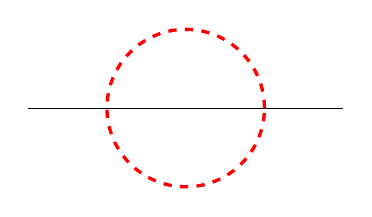
\begin{tikzpicture}
    % Draw a line from (0,0) to (4,0)
    \draw (0,0) -- (4,0);

    % Draw a dashed red circle with a center at (2,0) and a radius of 1cm
    \draw[dashed, red, very thick] (2,0) circle (1cm); 
\end{tikzpicture}
\end{center}

\subsection{Color, Fill, and Shading}
\begin{center}
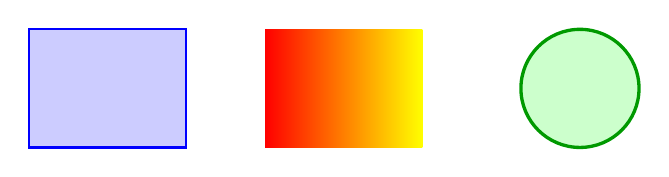
\begin{tikzpicture}
    % Solid fill
    \draw[draw=blue, fill=blue!20, thick] (0,0) rectangle (2,1.5);
    
    % Gradient shading
    \shade[left color=red, right color=yellow] (3,0) rectangle (5,1.5);
    
    % Circle with fill
    \draw[draw=green!60!black, fill=green!20, very thick] (7,0.75) circle (0.75cm);
\end{tikzpicture}
\end{center}

\subsection{Line Styles and Arrows}
\begin{center}
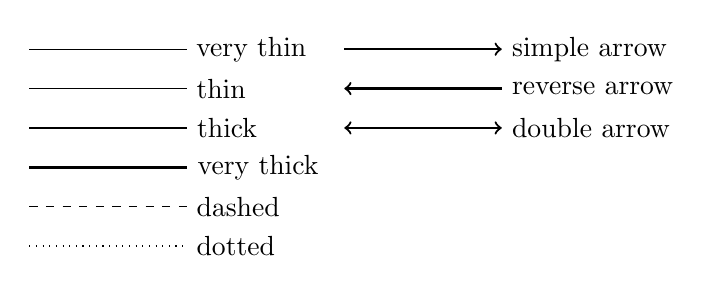
\begin{tikzpicture}
    % Different line thicknesses
    \draw[very thin] (0,3) -- (2,3) node[right] {very thin};
    \draw[thin] (0,2.5) -- (2,2.5) node[right] {thin};
    \draw[thick] (0,2) -- (2,2) node[right] {thick};
    \draw[very thick] (0,1.5) -- (2,1.5) node[right] {very thick};
    
    % Different line patterns
    \draw[dashed] (0,1) -- (2,1) node[right] {dashed};
    \draw[dotted] (0,0.5) -- (2,0.5) node[right] {dotted};
    
    % Arrows
    \draw[->, thick] (4,3) -- (6,3) node[right] {simple arrow};
    \draw[<-, thick] (4,2.5) -- (6,2.5) node[right] {reverse arrow};
    \draw[<->, thick] (4,2) -- (6,2) node[right] {double arrow};
\end{tikzpicture}
\end{center}

\subsection{Centering and Scaling}
\begin{center}
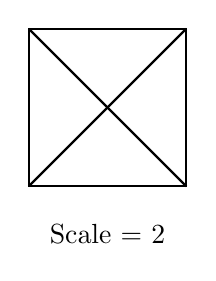
\begin{tikzpicture}[scale=2]
    % Scaled drawing - twice the normal size
    \draw[thick] (0,0) rectangle (1,1);
    \draw[thick] (0,0) -- (1,1);
    \draw[thick] (0,1) -- (1,0);
    \node at (0.5, -0.3) {Scale = 2};
\end{tikzpicture}
\end{center}

\section{Advanced Nodes and Positioning}
This section demonstrates advanced node usage, including text with math mode, anchored positioning, and relative placement.

\subsection{Nodes with Text and Math Mode}
\begin{center}
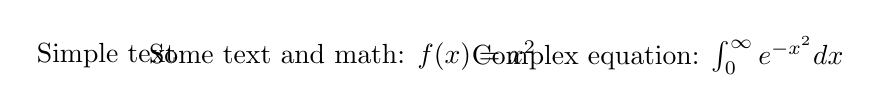
\begin{tikzpicture}
    % Node with text and math
    \node at (0, 0) {Simple text};
    \node at (3, 0) {Some text and math: $f(x) = x^2$};
    \node at (7, 0) {Complex equation: $\int_0^\infty e^{-x^2} dx$};
\end{tikzpicture}
\end{center}

\subsection{Anchored Nodes}
\begin{center}
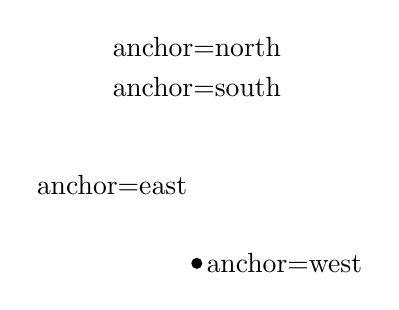
\begin{tikzpicture}
    % Reference point
    \fill (0,0) circle (2pt);
    
    % Nodes anchored at different positions
    \node[anchor=west] at (0,0) {anchor=west};
    \node[anchor=east] at (0,1) {anchor=east};
    \node[anchor=south] at (0,2) {anchor=south};
    \node[anchor=north] at (0,3) {anchor=north};
\end{tikzpicture}
\end{center}

\subsection{SIR Model Diagram with Styled Nodes}
This example demonstrates the SIR (Susceptible-Infected-Recovered) model using styled nodes and relative positioning.

\begin{center}
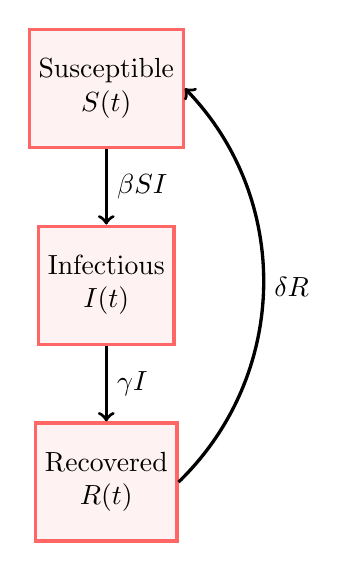
\begin{tikzpicture}[
    sir/.style={
        rectangle, 
        draw=red!60!white, 
        fill=red!5!white, 
        very thick, 
        minimum size=1.5cm,
        align=center
    },
    node distance=2.5cm 
]

    % Create the first node (Susceptible)
    \node[sir] (susceptible) {Susceptible \\ $S(t)$}; 

    % Create the second node (Infectious) positioned below the first
    \node[sir, below of=susceptible] (infectious) {Infectious \\ $I(t)$};
    
    % Create the third node (Recovered) positioned below the second
    \node[sir, below of=infectious] (recovered) {Recovered \\ $R(t)$};

    % Draw very thick arrows between the nodes
    \draw[->, very thick] (susceptible.south) -- (infectious.north) node[midway, right] {$\beta SI$};
    \draw[->, very thick] (infectious.south) -- (recovered.north) node[midway, right] {$\gamma I$};
    
    % Add a curved arrow from recovered back to susceptible (loss of immunity)
    \draw[->, very thick] (recovered.east) to[bend right=45] node[right] {$\delta R$} (susceptible.east);

\end{tikzpicture}
\end{center}

\subsection{Curved Arrows with B\'ezier Curves}
\begin{center}
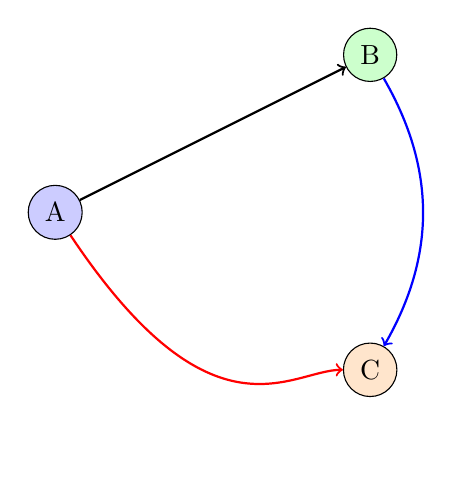
\begin{tikzpicture}
    % Define nodes
    \node[circle, draw, fill=blue!20] (A) at (0,0) {A};
    \node[circle, draw, fill=green!20] (B) at (4,2) {B};
    \node[circle, draw, fill=orange!20] (C) at (4,-2) {C};
    
    % Straight arrow
    \draw[->, thick] (A) -- (B);
    
    % Curved arrow using Bézier curve with control points
    \draw[->, thick, red] (A) .. controls (2,-3) and (3,-2) .. (C);
    
    % Smooth curve between two points
    \draw[->, thick, blue] (B) to[bend left=30] (C);
\end{tikzpicture}
\end{center}

\subsection{Complex Flow Diagram with Relative Positioning}
\begin{center}
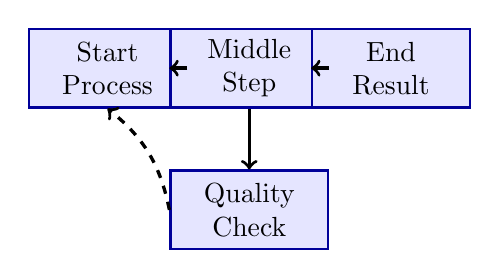
\begin{tikzpicture}[
    box/.style={rectangle, draw=blue!60!black, fill=blue!10, thick, minimum width=2cm, minimum height=1cm, align=center},
    node distance=1.8cm
]
    % Create nodes with relative positioning
    \node[box] (start) {Start \\ Process};
    \node[box, right of=start] (middle) {Middle \\ Step};
    \node[box, right of=middle] (end) {End \\ Result};
    \node[box, below of=middle] (check) {Quality \\ Check};
    
    % Connect nodes with arrows
    \draw[->, very thick] (start) -- (middle);
    \draw[->, very thick] (middle) -- (end);
    \draw[->, very thick] (middle) -- (check);
    \draw[->, very thick, dashed] (check.west) to[bend right=20] (start.south);
\end{tikzpicture}
\end{center}

\section{Flowcharts}
Here's a simple flowchart:

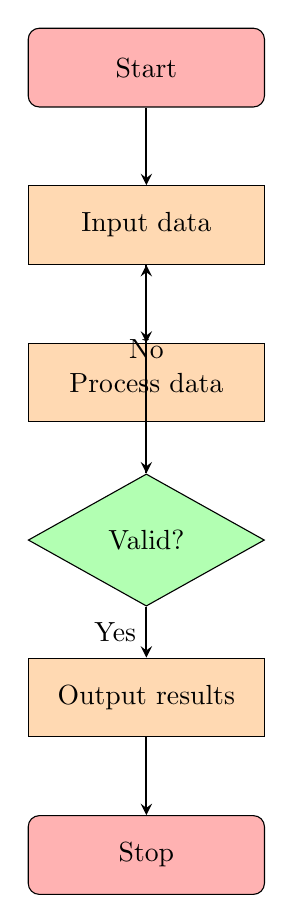
\begin{tikzpicture}[node distance=2cm]
% Define styles
\tikzstyle{startstop} = [rectangle, rounded corners, minimum width=3cm, minimum height=1cm, text centered, draw=black, fill=red!30]
\tikzstyle{process} = [rectangle, minimum width=3cm, minimum height=1cm, text centered, draw=black, fill=orange!30]
\tikzstyle{decision} = [diamond, minimum width=3cm, minimum height=1cm, text centered, draw=black, fill=green!30]
\tikzstyle{arrow} = [thick,->,>=stealth]

% Draw nodes
\node (start) [startstop] {Start};
\node (input) [process, below of=start] {Input data};
\node (process) [process, below of=input] {Process data};
\node (decision) [decision, below of=process] {Valid?};
\node (output) [process, below of=decision] {Output results};
\node (stop) [startstop, below of=output] {Stop};

% Draw arrows
\draw [arrow] (start) -- (input);
\draw [arrow] (input) -- (process);
\draw [arrow] (process) -- (decision);
\draw [arrow] (decision) -- node[anchor=east] {Yes} (output);
\draw [arrow] (decision) -- node[anchor=south] {No} (input);
\draw [arrow] (output) -- (stop);
\end{tikzpicture}

\section{Mathematical Plots}
Here's a mathematical plot:

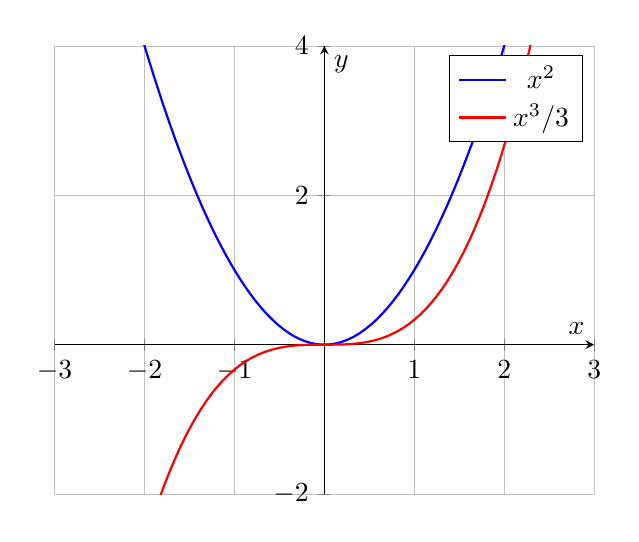
\begin{tikzpicture}
\begin{axis}[
    axis lines = center,
    xlabel = $x$,
    ylabel = $y$,
    xmin = -3, xmax = 3,
    ymin = -2, ymax = 4,
    grid = both,
    grid style = {line width=.1pt, draw=gray!10},
    major grid style = {line width=.2pt, draw=gray!50},
]
\addplot[domain=-3:3, samples=100, color=blue, thick] {x^2};
\addplot[domain=-3:3, samples=100, color=red, thick] {x^3/3};
\legend{$x^2$, $x^3/3$}
\end{axis}
\end{tikzpicture}

\section{Network Diagrams}
Here's a simple network diagram:

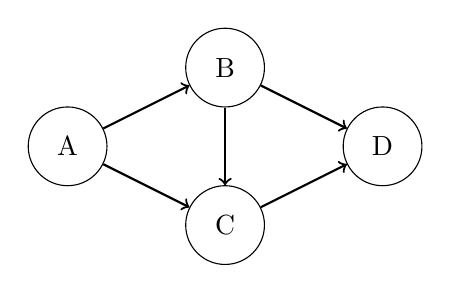
\begin{tikzpicture}[node distance=2cm]
% Define node styles
\tikzstyle{node} = [circle, draw, minimum size=1cm]
\tikzstyle{edge} = [thick, ->]

% Draw nodes
\node[node] (A) at (0,0) {A};
\node[node] (B) at (2,1) {B};
\node[node] (C) at (2,-1) {C};
\node[node] (D) at (4,0) {D};

% Draw edges
\draw[edge] (A) -- (B);
\draw[edge] (A) -- (C);
\draw[edge] (B) -- (D);
\draw[edge] (C) -- (D);
\draw[edge] (B) -- (C);
\end{tikzpicture}

\section{Advanced TikZ Features}
Here are some advanced TikZ features:

\subsection{Decorations}
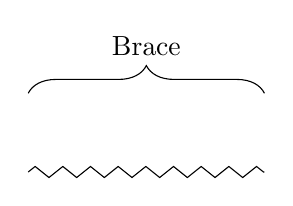
\begin{tikzpicture}
\draw[decorate, decoration={brace, amplitude=10pt}] (0,0) -- (3,0) node[midway, above=10pt] {Brace};
\draw[decorate, decoration={zigzag, amplitude=2pt}] (0,-1) -- (3,-1);
\end{tikzpicture}

\subsection{Shadows and Effects}
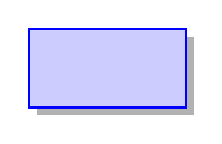
\begin{tikzpicture}
% Simulated drop shadow using a filled, slightly offset rectangle
\fill[black, opacity=0.3] (0.1,-0.1) rectangle (2.1,0.9);
\draw[fill=blue!20, draw=blue, thick] (0,0) rectangle (2,1);
\end{tikzpicture}

\section{Best Practices for TikZ}
\begin{itemize}
    \item Use relative coordinates when possible
    \item Define styles for consistent formatting
    \item Use meaningful node names
    \item Keep diagrams simple and clear
    \item Use appropriate line weights and colors
    \item Test diagrams at different scales
\end{itemize}

\section{Reference Examples from Dr. Trefor Bazett's Tutorial}
The following examples are directly from the tutorial video demonstrating key TikZ concepts.

\subsection{Example 1: Drawing and Styling a Circle}
This example demonstrates basic drawing commands and styling options:

\begin{center}
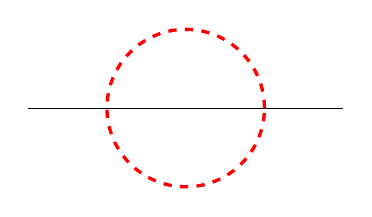
\begin{tikzpicture}
    % Draw a line from (0,0) to (4,0)
    \draw (0,0) -- (4,0);

    % Draw a dashed red circle with a center at (2,0) and a radius of 1cm
    \draw[dashed, red, very thick] (2,0) circle (1cm); 
\end{tikzpicture}
\end{center}

\subsection{Example 2: Defining and Using Custom Styles}
This example creates a reusable style called \texttt{sir} and then uses it to draw a diagram box with styled nodes:

\begin{center}
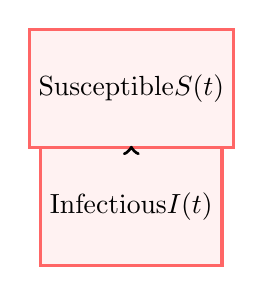
\begin{tikzpicture}[
    sir/.style={
        rectangle, 
        draw=red!60!white, 
        fill=red!5!white, 
        very thick, 
        minimum size=1.5cm
    },
    % Positioning library is required for 'below of'
    node distance=1.5cm 
]

    % Create the first node (Susceptible)
    \node[sir] (susceptible) {Susceptible \\ $S(t)$}; 

    % Create the second node (Infectious) positioned below the first
    \node[sir, below of=susceptible] (infectious) {Infectious \\ $I(t)$};

    % Draw a very thick arrow between the two nodes
    \draw[->, very thick] (susceptible.south) -- (infectious.north);

\end{tikzpicture}
\end{center}

\end{document}
